\documentclass[12pt, titlepage]{article}

\usepackage{fullpage}
\usepackage[round]{natbib}
\usepackage{multirow}
\usepackage{booktabs}
\usepackage{tabularx}
\usepackage{graphicx}
\usepackage{float}
\usepackage{hyperref}
\usepackage{float}
\hypersetup{
    colorlinks,
    citecolor=blue,
    filecolor=black,
    linkcolor=red,
    urlcolor=blue
}

%% Comments

\usepackage{color}

\newif\ifcomments\commentstrue %displays comments
%\newif\ifcomments\commentsfalse %so that comments do not display

\ifcomments
\newcommand{\authornote}[3]{\textcolor{#1}{[#3 ---#2]}}
\newcommand{\todo}[1]{\textcolor{red}{[TODO: #1]}}
\else
\newcommand{\authornote}[3]{}
\newcommand{\todo}[1]{}
\fi

\newcommand{\wss}[1]{\authornote{blue}{SS}{#1}} 
\newcommand{\plt}[1]{\authornote{magenta}{TPLT}{#1}} %For explanation of the template
\newcommand{\an}[1]{\authornote{cyan}{Author}{#1}}

%% Common Parts

\newcommand{\progname}{ProgName} % PUT YOUR PROGRAM NAME HERE
\newcommand{\authname}{Team \#, Team Name
\\ Student 1 name and macid
\\ Student 2 name and macid
\\ Student 3 name and macid
\\ Student 4 name and macid} % AUTHOR NAMES                  

\usepackage{hyperref}
    \hypersetup{colorlinks=true, linkcolor=blue, citecolor=blue, filecolor=blue,
                urlcolor=blue, unicode=false}
    \urlstyle{same}
                                


\newcounter{acnum}
\newcommand{\actheacnum}{AC\theacnum}
\newcommand{\acref}[1]{AC\ref{#1}}

\newcounter{ucnum}
\newcommand{\uctheucnum}{UC\theucnum}
\newcommand{\uref}[1]{UC\ref{#1}}

\newcounter{mnum}
\newcommand{\mthemnum}{M\themnum}
\newcommand{\mref}[1]{M\ref{#1}}

\begin{document}

\title{System Design for \progname{}} 
\author{\authname}
\date{\today}

\maketitle

\pagenumbering{roman}

\section{Revision History}

\begin{tabularx}{\textwidth}{p{3cm}p{2cm}X}
\toprule {\bf Date} & {\bf Version} & {\bf Notes}\\
\midrule
18 January 2023 & 1.0 & Revision 0 for System Design\\
\bottomrule
\end{tabularx}

\newpage

\section{Reference Material}

This section records information for easy reference.

\subsection{Abbreviations and Acronyms}

\renewcommand{\arraystretch}{1.2}
\begin{tabular}{l l} 
  \toprule		
  \textbf{symbol} & \textbf{description}\\
  \midrule 
  \progname & Explanation of program name\\
  \wss{...} & \wss{...}\\
  \bottomrule
\end{tabular}\\

\newpage

\tableofcontents

\newpage

\listoftables

\listoffigures

\newpage

\pagenumbering{arabic}

\section{Introduction}

\wss{Include references to your other documentation}

\section{Purpose}

\wss{Purpose of your design documentation}

\wss{Point to your other design documents}

\section{Scope}

\wss{Include a figure that show the System Context (showing the boundary between
your system and the environment around it.)}

\section{Project Overview}

\subsection{Normal Behaviour}

\subsection{Undesired Event Handling}

\wss{How you will approach undesired events}

\subsection{Component Diagram}

\subsection{Connection Between Requirements and Design} \label{SecConnection}

\wss{The intention of this section is to document decisions that are made
  ``between'' the requirements and the design.  To satisfy some requirements,
  design decisions need to be made.  Rather than make these decisions implicit,
  they are explicitly recorded here.  For instance, if a program has security
  requirements, a specific design decision may be made to satisfy those
  requirements with a password.}

\section{System Variables}

\wss{Include this section for Mechatronics projects}

\subsection{Monitored Variables}

\subsection{Controlled Variables}

\subsection{Constants Variables}

\section{User Interfaces}

\subsection{Hardware User Interface}

The device is worn by a participant on the wrist for measuring activity and generating  prompts. The following items will be shown on the display of the activity tracker:
\begin{table}[H]
	\begin{tabularx}{1.05\textwidth} { 
		  | >{\centering\arraybackslash}X 
		  | >{\centering\arraybackslash}X 
		  | >{\centering\arraybackslash}X 
		  | >{\centering\arraybackslash}X | }
		 \hline
		 Description & Behaviour of TFT Display \\
		 \hline
		Power up of activity tracker. & Displays Back End Developers on startup.\\
		\hline
		 Default behaviour, no activity tracked.  & Displays date and time.\\
		 \hline
		   Activity tracked. & Prompt generated on screen, for example: Are you in pain?\\
		\hline 
		Answering prompts using touch sensor (bezel). & Toggle between different 				options on screen. For example: (Yes/No).\\
		\hline
	\end{tabularx}
\caption{\label{Hardware User Interface}Components of Hardware User Interface}  
\end{table}

\begin{figure}[H]
	\begin{center}
		 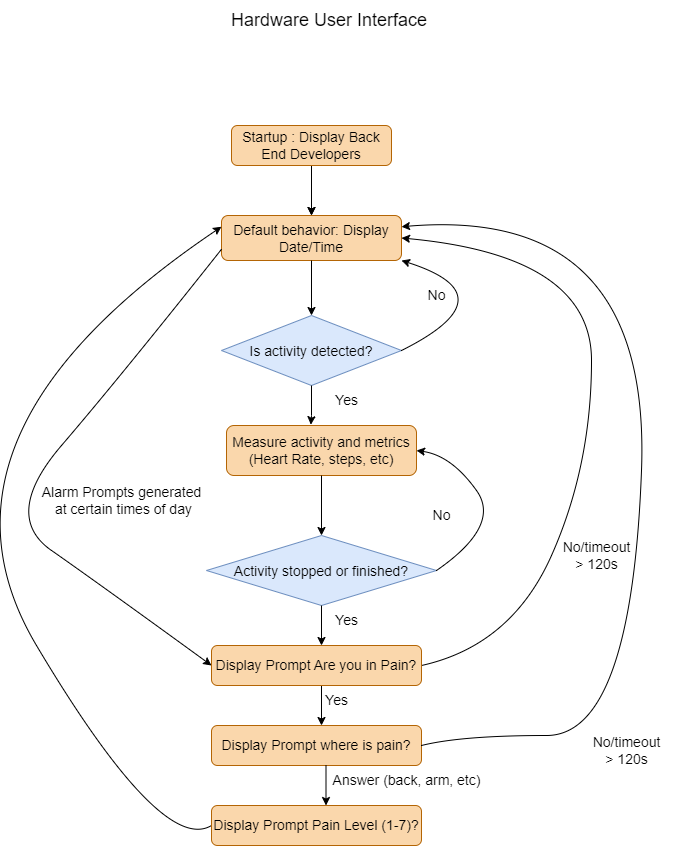
\includegraphics[width=1\textwidth]{HardwareUI_FSM}
		\caption{Finite State Machine for Hardware User Interface}
		\label{HardwareUI_FSM} 
	\end{center}
\end{figure}

\subsection{Software User Interface}

The Software User Interface will be used by the Researcher for configuring the activity tracker according to the participant. The interface will be on the Host Computer and will be able to store participant data, create new data and view records using encryption. The interface will also have authentication, and only the Researcher will be able to log in. The following features are available on the Software User Interface:

\begin{table}[H]
	\begin{tabularx}{1.05\textwidth} { 
		  | >{\centering\arraybackslash}X 
		  | >{\centering\arraybackslash}X 
		  | >{\centering\arraybackslash}X 
		  | >{\centering\arraybackslash}X | }
		 \hline
		 Options on UI & Description\\
		 \hline
		Main window & Main menu that leads to different windows when clicked.\\
		\hline
		 Connect to tracker  & Connects to SD card for device and shows status of connection.\\
		 \hline
		   Create Records Window & Creates new record for particpant and stores it in a database. A record can only be created if the correct username and password is provided. \\
		\hline 
		Records Window & Participant records can be viewed in a tabular format and can be searched/filtered.\\
		\hline
		Data View Window & Data stored on SD card can be viewed and filtered. Data can also be plotted using Graph button. For example: Heart Rate vs Time.\\
		\hline
	\end{tabularx}
\caption{\label{Software User Interface}Components of Software User Interface}  
\end{table}

Below is an example of the Software User Interface for the Main window.
\begin{figure}[H]
	\begin{center}
		 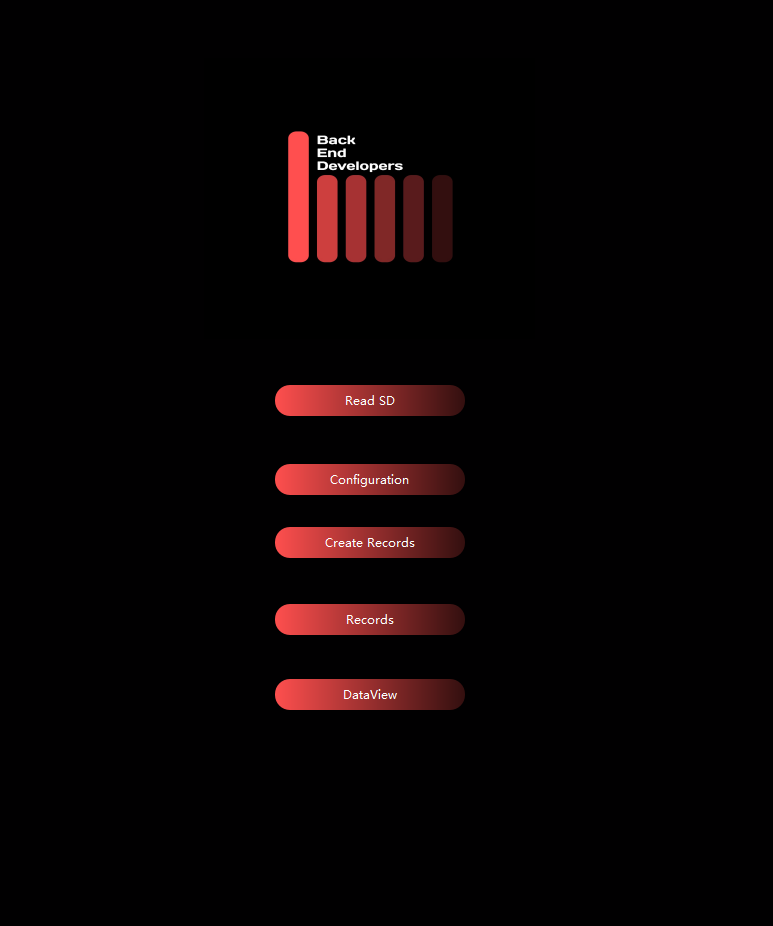
\includegraphics[width=0.8\textwidth]{MainWindow}
		\caption{Main Window}
		\label{MainWindow} 
	\end{center}
\end{figure}

For more examples of Software User Unterface, refer to Appendix.

\begin{figure}[H]
	\begin{center}
		 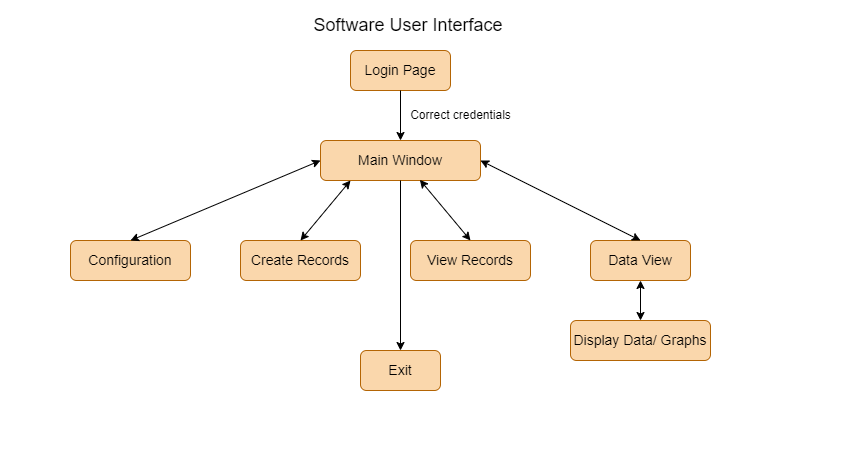
\includegraphics[width=1\textwidth]{SoftwareUI_FSM}
		\caption{Finite State Machine for Software User Interface}
		\label{SoftwareUI_FSM} 
	\end{center}
\end{figure}

\wss{Design of user interface for software and hardware.  Attach an appendix if
needed. Drawings, Sketches, Figma}

\section{Design of Hardware}

The table below shows hardware components that will be used in the activity tracker.
\begin{table}[H]
	\begin{tabularx}{1.05\textwidth} { 
		  | >{\centering\arraybackslash}X 
		  | >{\centering\arraybackslash}X 
		  | >{\centering\arraybackslash}X 
		  | >{\centering\arraybackslash}X | }
		 \hline
		 \textbf{Hardware Component} & \textbf{Description}\\
		 \hline
		Custom PCB & Custom PCB designed to fit in activity tracker.  \\
		\hline 
		 MPU 6050 & Accelrometer/Gyroscope, off-shelf component.\\
		\hline
		 seeeduino xiao samd21  & off-shelf microcontroller for activity tracker.\\
		 \hline
		   DS1307 RTC & Real time clock, off-shelf component. \\
		\hline
		TFT Display & Off-shelf display used in activity tracker. \\
		\hline 
		Outer casing for TFT Display & Designed using Autodesk Inventor and 3D printed \\
		\hline 
		Li-Po Battery & Generic off-shelf lipo battery used for smart watches.  \\
		\hline 
		USB Type-B charger & Generic off-shelf usb to Type-B charger to charge device. \\
		\hline 
		MicroSD card & Standard off-shelf SD card. \\
		\hline
		SDCARD connector 473521001& MicroSD connector (off-shelf component) \\
		\hline
		Watch straps & Generic watch-straps for strapping device onto the wrist. \\
		\hline 
	\end{tabularx}
\caption{\label{DesignHardware}Components of Hardware Design}  
\end{table}

\wss{Most relevant for mechatronics projects}
\wss{Show what will be acquired}
\wss{Show what will be built, with detail on fabrication and materials}
\wss{Include appendices as appropriate, possibly with sketches, drawings, CAD, etc}

\section{Design of Electrical Components}

\wss{Most relevant for mechatronics projects}
\wss{Show what will be acquired}
\wss{Show what will be built, with detail on fabrication and materials}
\wss{Include appendices as appropriate, possibly with sketches, drawings,
circuit diagrams, etc}

\section{Design of Communication Protocols}

\wss{If appropriate}

\section{Timeline}

\wss{Schedule of tasks and who is responsible}

% \bibliographystyle {plainnat}
% \bibliography{../../../refs/References}

\newpage{}

\appendix

\section{Software Interface}

\begin{figure}[H]
	\begin{center}
		 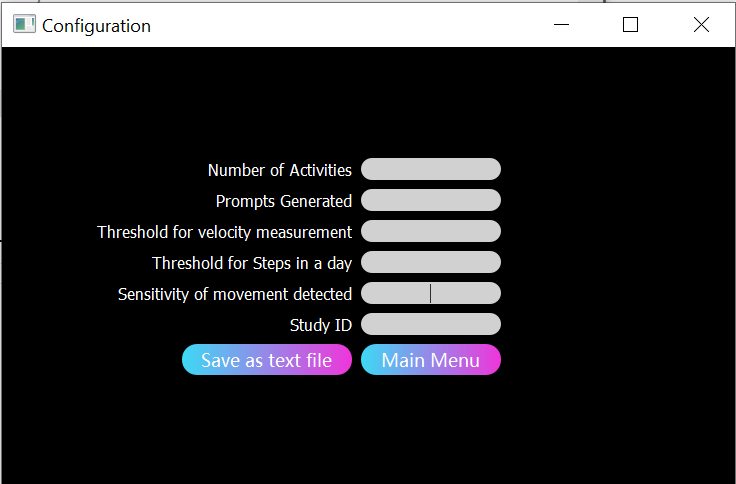
\includegraphics[width=0.8\textwidth]{Config}
		\caption{Configuration Window}
		\label{Config} 
	\end{center}
\end{figure}

\begin{figure}[H]
	\begin{center}
		 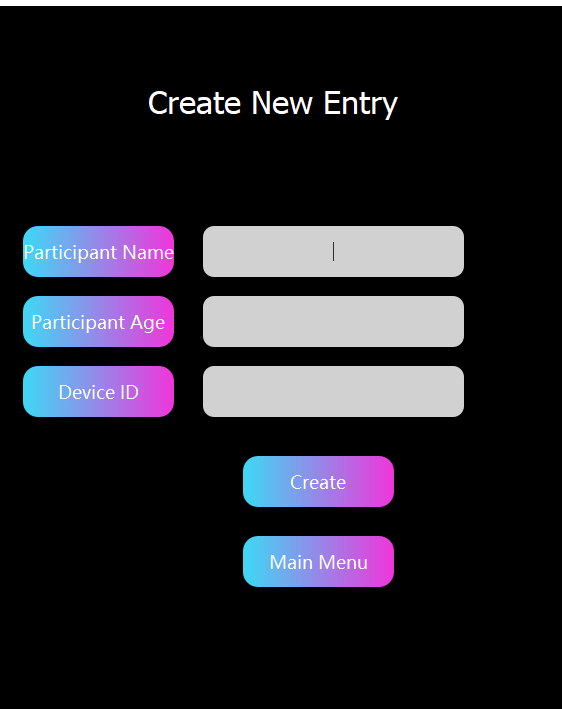
\includegraphics[width=0.5\textwidth]{CreateRecord}
		\caption{Create Record Window}
		\label{CreateRecord} 
	\end{center}
\end{figure}

\begin{figure}[H]
	\begin{center}
		 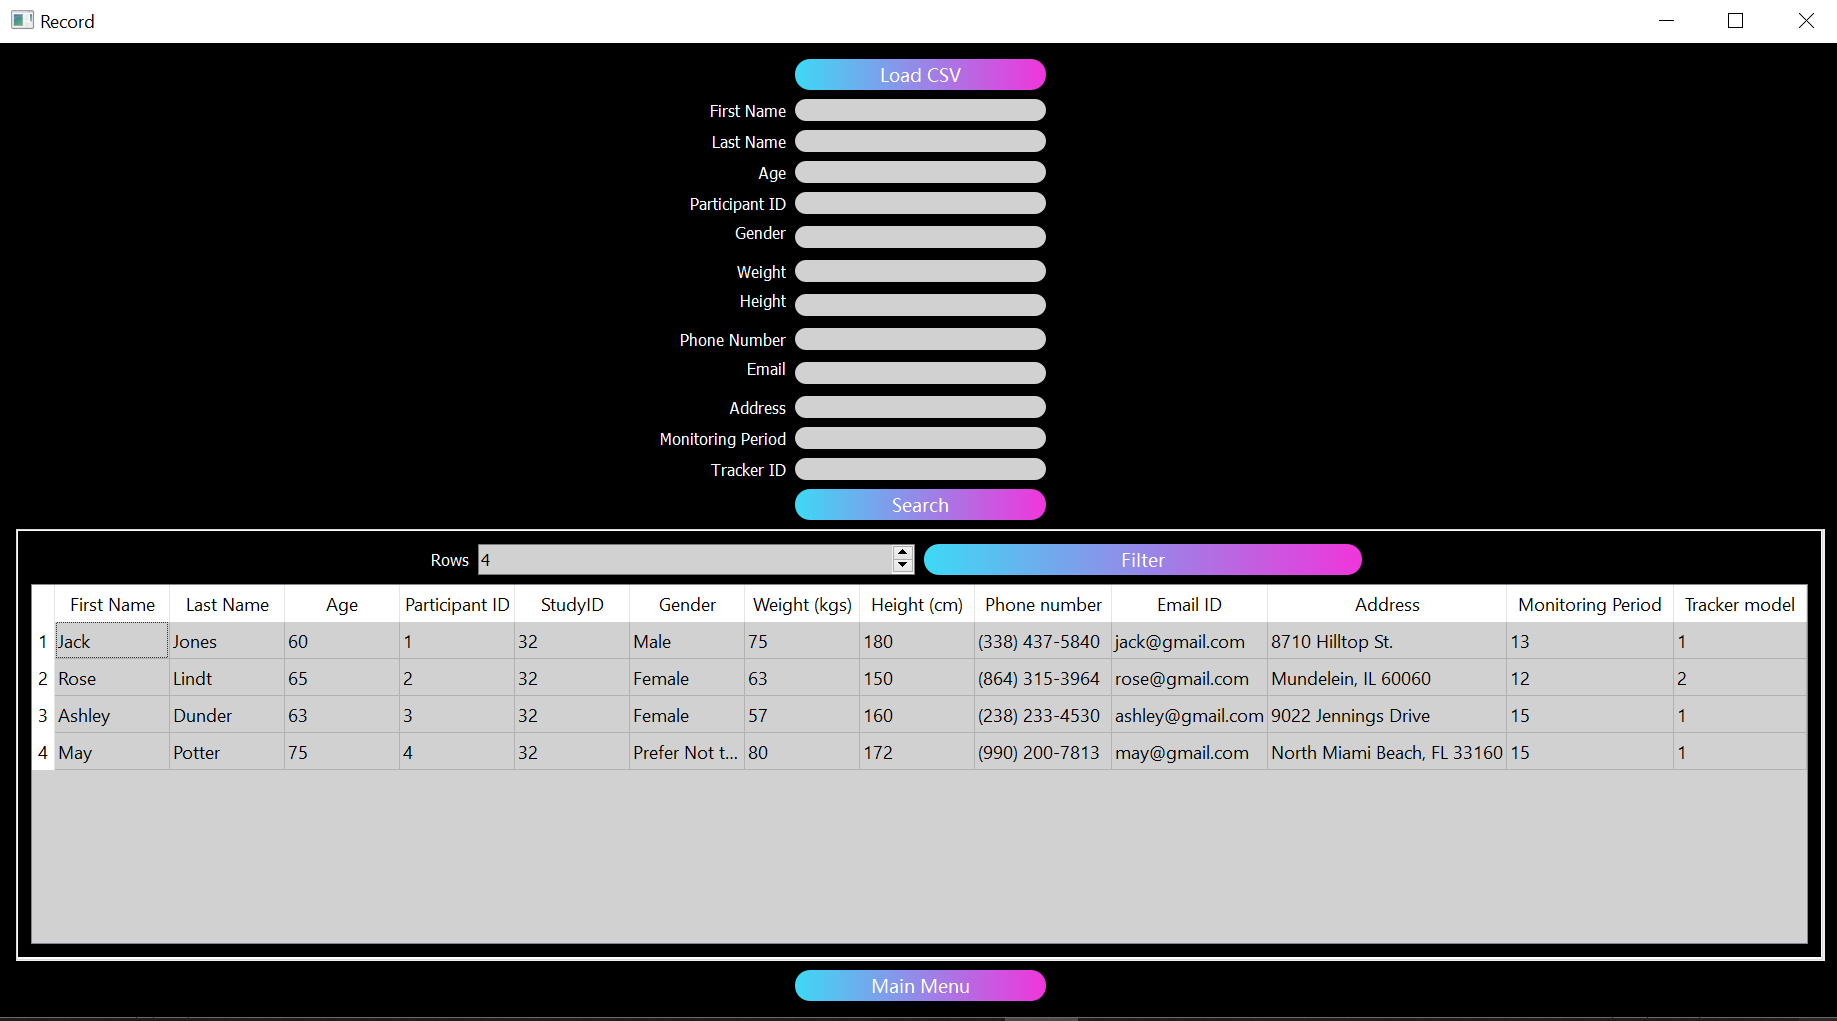
\includegraphics[width=1\textwidth]{Record}
		\caption{Record Window}
		\label{Record} 
	\end{center}
\end{figure}

\begin{figure}[H]
	\begin{center}
		 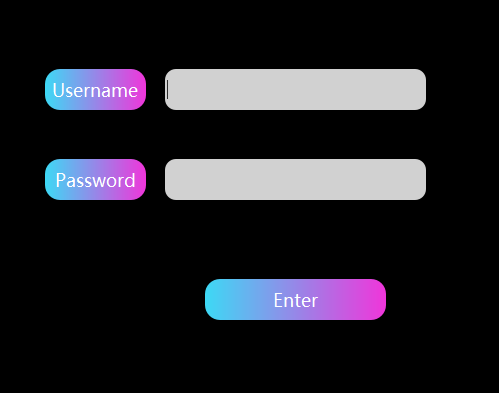
\includegraphics[width=0.5\textwidth]{login}
		\caption{Login Dialogue box}
		\label{Login} 
	\end{center}
\end{figure}

\begin{figure}[H]
	\begin{center}
		 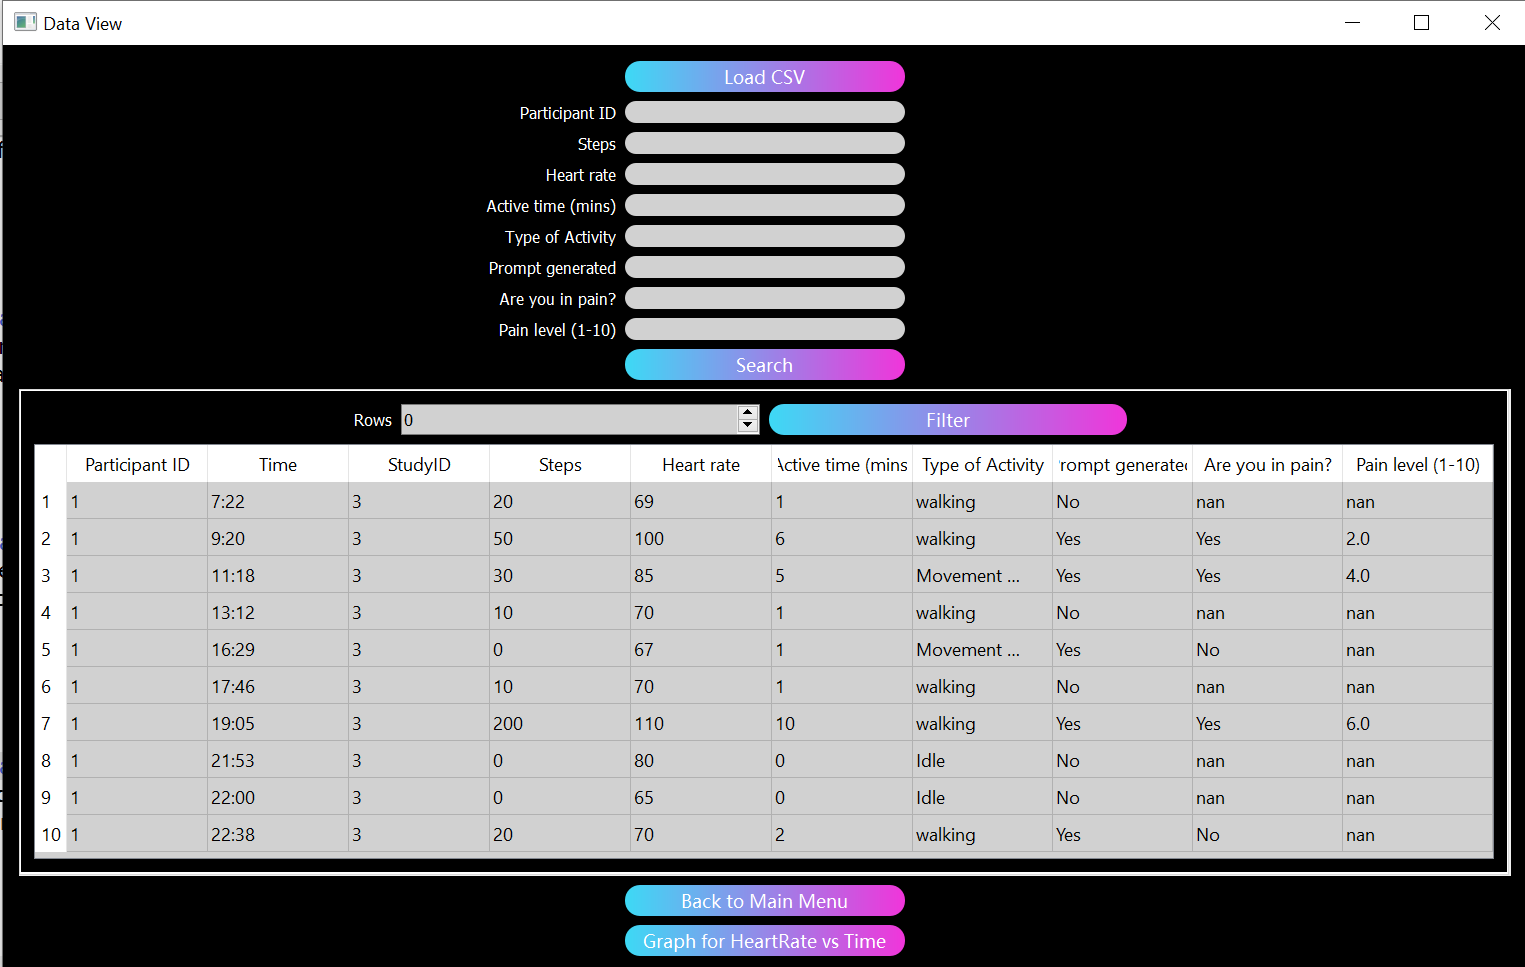
\includegraphics[width=1\textwidth]{DataView}
		\caption{Data View Window}
		\label{DataView} 
	\end{center}
\end{figure}

\begin{figure}[H]
	\begin{center}
		 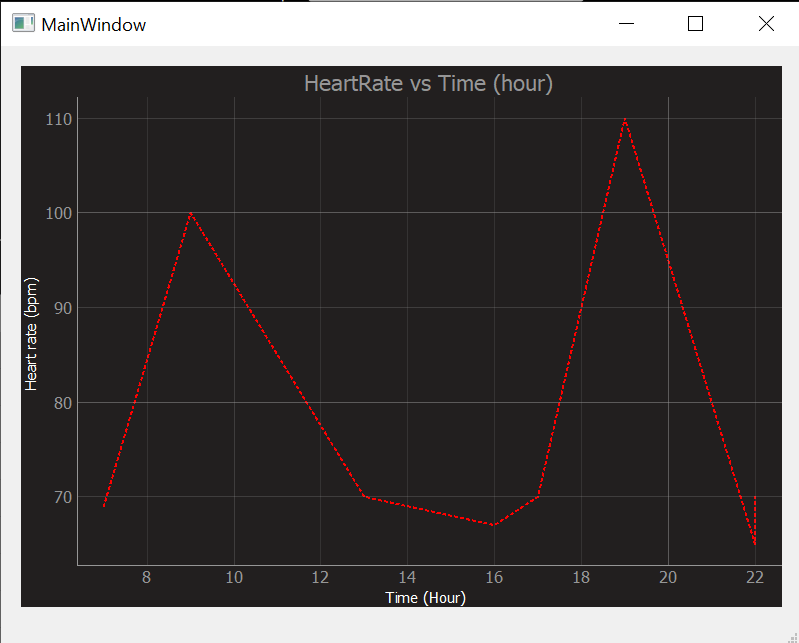
\includegraphics[width=0.8\textwidth]{Graph}
		\caption{Generated Graph for Heart Rate vs Time}
		\label{Graph} 
	\end{center}
\end{figure}
\section{Mechanical Hardware}

\section{Electrical Components}

\section{Communication Protocols}

\section{Reflection}

The information in this section will be used to evaluate the team members on the
graduate attribute of Problem Analysis and Design.  Please answer the following questions:

\begin{enumerate}
  \item What are the limitations of your solution?  Put another way, given
  unlimited resources, what could you do to make the project better? (LO\_ProbSolutions)
  \item Give a brief overview of other design solutions you considered.  What
  are the benefits and tradeoffs of those other designs compared with the chosen
  design?  From all the potential options, why did you select documented design?
  (LO\_Explores)
\end{enumerate}


\end{document}